%!TEX root = Manuscript.tex

\chapter{Scheduling Synchronized Periodic Datagrams in Arbitrary Networks }
\label{chap:SPALL}
\minitoc

In this chapter, we consider problem similar to \pall with an additional constraint : the sending of the messages in all the sources of the routes must be \textbf{synchronized}. This constraints brings us to allow the buffuring in every contention points of the nodes, in order to manage the datagrams to avoid collisions. Indeed, by allowing buffuring in every contention points of the routed network network (and not only in the one corresponding to the BBU), we have an higher degree of liberty to schedule the datagrams.

To do so, we modify the model in order to take into account the buffers, and we define the problem \textbf{S}ynchronized \textbf{P}eriodic \textbf{A}ssignment for \textbf{L}ow \textbf{L}atency (\spall). The algorithm presented in this section solves not only the star shaped network, but every directed acyclic multigraphs representing a routed network. We first show that the greedy algorithms principles used for star shaped networks are not efficient in routed network of higher contention depth, then we present some local search heuristics (hill climbing, simulated annealing, tabu search) that helps to solve the problem, and we present an FPT algorithm that gives the optimal solution, for which the exponential parameters are the number of routes and the contention depth of the routed network.

\todo{expliquer que buffuriser au debut ou au milieu c'est pareil donc que ca couvre PALL ? ou regarder ce que ca donnerais avec la metrique PALL}.


\section{Model changes}
\todo{Routed network pas exactement défini pareil.}
As a reminder, the  \textbf{contention depth} of a routed network $N = ({\cal R},\,{\cal B},\,\omega)$ is the maximal number of contention points on a route in the routed network. 

In the previous chapter, the set of vertices in which the buffering was allowed was denoted by ${\cal B}$. Here, we define by ${\cal C}$ the set of its contention vertices, in which buffering is allowed in each vertices. 
In the previous chapter, every routes in $\mathcal{R}$ had the same contention points $c_1$ and $c_2$. Since it is not the case anymore in this chapter, we define $\mathcal{R}_c$ the subset of routes in $\mathcal{R}$ belonging to $c$
Let $r \in {\cal R}$, with $r = (s,c_1,\dots,c_l,t)$, then we say that $c_i$ is of \textbf{contention level} $i$ for the route $r$, and we denote it by $cl(c_i,r) = i$. The contention level of a contention point $c$ is the maximum of its contention level over all routes going through itself: 
	$cl(c) = \max\limits_{r\in{\cal R}_c \text{ and } c \in r} cl(c,r)$.


   Let $r=(s,c_0,\dots,c_l,t)$ be a route. As mentioned above, in order to avoid contention, it is possible to buffer datagrams in contention points. The function $A$, called an \textbf{assignment}, associates an integer value, greater or equal to $0$, to each couple (route,vertex) of the routed network $N = ({\cal R},\,{\cal C},\,\omega)$. Those integers represent the buffering time of the datagrams in the contention points of the network: a datagram of route $r$ waits $A(r,c)$ tics in the buffer of $c$.
          
       

 The \textbf{arrival time} of a datagram in vertex $u_i$ of $r$, is the first time at which the datagram sent on $r$ reaches $u_i$, and is defined by $t(r,u_i) = \lambda(r,u_i) + \sum_{k=0}^{i-1} A(r,u_k) $. The date at which a datagram reaches a vertex $u_i$ is decomposed into a \emph{physical delay} due to the time to go through the links before $u_i$ and a \emph{logical} delay caused by the use of buffers as determined by assignment $A$.
  The \textbf{sending time} of a datagram at vertex $u_i$ of $r$, is the first time at which the datagram is sent by $u_i$. It is defined by $s(r,u_i) = t(r,u_i) +  A(r,u_i) $. This is the arrival time of the datagram plus the buffer time given by $A$.
 
  Consider $t$ the last vertex of the route $r$, the transmission time of the datagram on 
  $r$ is denoted by $TR(A,r)$ and is equal to $t(r,t)$. We define the \textbf{transmission time} of an assignment $A$ as $TR(A) = \displaystyle \max\limits_{r \in {\cal R}} TR(A,r) $. This is the time elapsed before the reception of the beginning of the last datagram. 

We then define the following problem :

 \noindent {\bf Synchronized Periodic Assignment for Low Latency (\spall)} 

      \noindent {\bf Input:}  Symmetric routed network $N = ({\cal R},\,{\cal C},\,\omega)$, period $P$, datagram size $\tau$ and a deadline function $d$.%, a bound on the latency $T$.
      
      %\noindent {\bf Decision problem:} is there a valid assignment $A$ of $(G,{\cal R})$ such that $ TR(A) \leq T$ ?

      \noindent {\bf Output:} assignment $A$ which minimizes $TR(A)$.
      \\
    
    Several parameters are important for the study of \spall. The algorithms we present have a complexity
    depending on $n$ the number of routes and $d$ the contention level. We evaluate the arithmetic complexity of our algorithms, that is arithmetic operations are considered to be in constant time. Then, the complexity will surprisingly not depend on $P$, $\tau$ or the weights of the routed network.

 \begin{theorem}\label{th:spallHard}
The problem $\spall$ is $\NP$-hard, even in routed networks of conflict depth $2$ (star shaped network)
\end{theorem}
\begin{proof}
The two flow shop problem studied in~\cite{yu2004minimizing} is shown to be $\NP$-hard. The problem is as follows, a set of jobs have to be processed in sequence on two machines; a job must be processed on machine $1$ before beeing processed on machine $2$. There is, for each job, a delay between the end of the processing on the first machine and the begining of the processing on the second one. The objective is to minimize the makespan. The time needed to process each job is the same.\\
We reduce an instance of $\spall$ in an instance of the two flow shop proplem: A message is a job, the delay of the jobs are equivalent to the lenght of the routes between the two contention points. We then set the makespan value to $P$, and the instance of $\spall$ becomes an instance of two flow shop.
\end{proof}


  \todo{petit bout sur l'explication qu'on ne considère pas le buffuring dans le Datacenter}


\section{Compact Representation of an Assignment}

 We define $\prec$, the pointwise order on assignments: $A_1 \preceq A_2$ if for all $r\in {\cal R}$, $TR(A_1,r) \leq TR(A_2,r)$. Moreover, we say that $A_1 \prec A_2$ if $A_1 \preceq A_2$ and there is an $r \in \cal {R}$ such that  $TR(A_1,r) < TR(A_2,r)$. Remark that assignments which minimize $TR(A)$ are also minimal for $\prec$. Hence, it is enough to consider minimal assignments for $\prec$ to solve \spall.

We explain in this section how to represent most assignment in a compact way, forgetting about the precise buffering time by only considering informations about the order of the datagrams in each contention point. All minimimal assignments have a compact representation, which implies that we do not need to consider assignment without a compact representation when solving \spall. 
It allows to design an FPT algorithm for \spall by going through all compact representations, but also to design good polynomial time heuristics using taboo search or simulated annealing, since one can easily define the neighborood of a compact representation.


\begin{definition}[Compact assignment]
Let $(G, \mathcal{R})$ be a routed network. A compact assignment $CA$ is a function which maps to each contention point $c$ in $G$ a pair $(O_c,S_c)$, where $O_c$ is an order on $\mathcal{R}_c$ and $S_c$ is a subset of $\mathcal{R}_c$.
\label{definition:compact}
\end{definition}


\subsection{From a Valid Assignment to its Compact Representation}

Let us define a function which maps a valid assignment $A$ to a compact assignment, called the compact representation of $A$, denoted by $CR(A)$. Let assume that for all contention vertices $u$, there is a route $r \in \mathcal{R}_u$ such that $A(r,u) = 0$.

We assume that routes in $\mathcal{R}$ are indexed by the integers in $[n]$. Say w.l.o.g. that $r_0$ is the route of smallest index such that $A(r_0,u) = 0$. The datagram of $r_0$ arrives, and goes to the next contention vertex, at time $t(r_0,u)$. Let us define the \textbf{normalized arrival time} of $r$ at $u$: for all $r \in \mathcal{R}_u$, $nt(r_0,r,u) = (t(r,u) - t(r_0,u)) \mod P$. It is the time at which the datagram of $r$ arrives at $u$, in a period normalized so that the datagram of $r_0$ goes through $u$ at time $0$. Similarly, we define the \textbf{normalized sending time} as $ns(r_0,r,u) = (s(r,u) - t(r_0,u)) \mod P$.

We define $O_u$ as the order on the routes of $\mathcal{R}_u$ induced by the values $ns(r,u)$. The set $S_u$ is defined as the set of routes going through $u$ such that $ns(r_0,r,u) < nt(r_0,r,u)$. Represent the time as cut into periods $[t(r_0,u) + iP,t(r_0,u) + (i+1)P [$ with $i \in \mathbb{N}$. Intuitively, $S_u$ represents the set of routes with a datagram going through $u$ in the period \emph{after} the one it has been available in. 

Fig.~\ref{fig:normalizedassignment} illustrates how a compact representation is computed from an assignment on a single node $u$. On top, the datagrams are represented by sending time $s(r_i,u)$ while the bottom of the figure shows the datagrams in a single period, represented by normalized sending times $ns(r_0,r_i,u)$.  
\begin{figure}[!h]
	\centering
	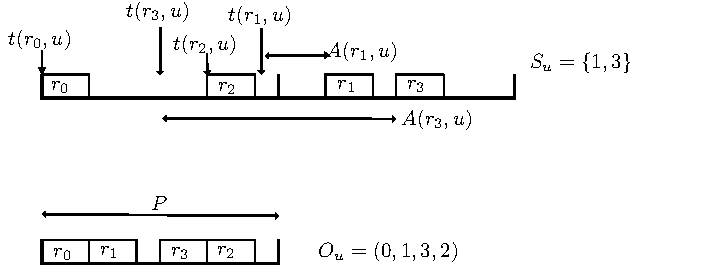
\includegraphics[scale=1]{Chapitre5/normalizedassignment}
\caption{A compact representation of an assignment in which $O_u = (0,1,3,2)$ and $S_u = \{1,3\}$ }
\label{fig:normalizedassignment}
\end{figure}


Note that for $CR(A)$ to be defined, we need that, on each contention point, at least a datagram is not buffered. We call such an assignment a \textbf{canonical assignment}. It turns out that any assignment $A$ can be made canonical without increasing $TR(A)$.

\begin{lemma}\label{lemma:canonical_min}
Let $A$ be a valid assignment, then there is a valid canonical assignment $A'$ such that $A' \preceq A$.
\end{lemma}
\begin{proof}
Consider a vertex $u$ of contention level $1$, such that for all $r \in \mathcal{R}_u$, $A(r,u) > 0$. Let us define $m$ as the minimum of these values, we define $A'(r,u) = A(r,u) - m$. Assignment $A'$ has no collision on $u$, since all departure times have been shifted by the same value and $A$ has no collision. Moreover, if $v$ is the vertex after $u$ in a route $r$, we define  $A'(r,v) = A(r,v) + m$. Hence, all departure times for vertices of contention levels larger than one are the same in $A$ and $A'$, which implies that there are no collisions in these vertices. We have proven that $A'$ is still valid. Since all departure times of $A'$ are less or equal to those induced by $A$, we have $A' \preceq A$. Moreover, if $r_0$ is the route with $A(r_0,u) = m$, then $A'(r_0,u) = 0$. 

We apply this transformation by increasing contention level. Since, the transformation applied at some contention level do not change $A'$ for smaller contention levels, a trivial induction proves that $A'$ is valid, canonical and that $A' \preceq A$.
\end{proof}


\subsection{From a Compact Assignment to its Realization}\label{sec:real}


We now explain how to transform a compact representation into a canonical assignment.
Moreover, we show that the obtained assignment is the smallest among all assignments of same representation. We first explain how to do the transformation on a routed network with a single contention vertex $u$.

Recall that the datagram of a route $r$ is available at time $t(r,u)$ in the vertex $u$.
Let us consider a compact assignment $CA$, which maps $u$ to the pair $(O_u,S_u)$.
The assignment $Real(CA)$ is built inductively from $CA$, it is called the realization of $CA$. 
If the construction of $Real(CA)$ fails, then $Real(CA)$ is undefined and we say that $CA$ is not realizable. In the next paragraph, we build an assignment $A$ by setting the buffering time of the routes in the order
 $(O_u)$. If the construction suceeds, we set $Real(CA) = A$ 

Let say that the order $O_u$ is $(r_0, \dots, r_l)$. We fix $A(r_0,u)$ to zero, that is the first
datagram in the period has no buffering time. Then, in each period beginning by the first datagram, the datagrams will be in order $O_u$. When the first datagram of the period is chosen, we use it to define normalized arrival times and normalized sending times.
Assume that $A(r_i,u)$ have been set for $i \leq l$, let us explain how to 
set $A(r_{i+1},u)$. If $r_{i+1} \notin S_u$, then $A(r_{i+1},u)$ is chosen so that $ns(r_1,r_{i+1},u)$ is the maximum of $ns(r_1,r_i,u) + \tau$ and $nt(r_1,r_{i+1},u)$. If $ns(r_1,r_{i+1},u) > P - \tau$, then $CA$ is not realizable. If $r_{i+1} \in S_u$, then $A(r_{i+1},u)$ is chosen so that $ns(r_1, r_{i+1},u) = ns(r_1,r_i,u) + \tau$. In both cases, if $ns(r_1, r_{i+1},u) \geq nt(r_1,r_{i+1},u)$, then $CA$ is not realizable (the sending time is in the wrong period with regard to $S_u$). 

Figure~\ref{fig:compacttoassignment} shows how an assignment $Real(CA)$ is built from a compact assignment $CA$ on a single contention vertex $u$. We have $O_u = (2,1,0,3)$ and $S_u = \{1\}$. First, the datagram $2$ is fixed, that is, $A(r_2,u)=0$. Then, since $r_1 \in S_u$, we set $A(r_1,u)$ such that $ ns(r_2,r_1,u) = ns(r_2,r_2,u) + \tau$. 
Finally, since $r_0$ and $r_3 \notin S_u$, we set $A(r_0,u)$ and $A(r_3,u)$ such that $ns(r_2,r_0,u) = nt(r_2,r_0,u)$ and  $ns(r_2,r_3,u) = ns(r_2,r_0,u) + \tau$.
\begin{figure}[!h]
	\centering
	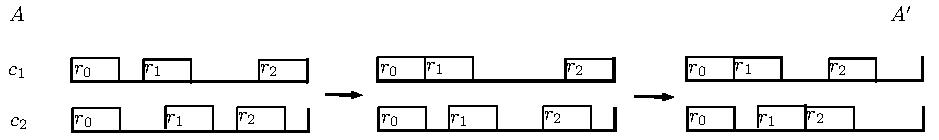
\includegraphics[scale=1]{Chapitre5/compacttoassignment}
\caption{Inductive construction of $Real((2,1,0,3),\{1\})$ from $CA$ on a single contention vertex $u$. }
\label{fig:compacttoassignment} 
\end{figure}

The function $Real$ can easily be generalized to any routed network. Indeed, one can first consider all vertices of contention level $1$, the routes going through them form disjoint sets. Hence, we can define $Real$ independently on each vertex of contention level $1$. 
Then using the buffering computed for this vertices, one can compute the arrival time of each route in vertices of contention level $2$ and compute $Real$ for these vertices in the exact same way, and so on for all contention levels. In the following lemmas and theorems, we always consider a single contention vertex, since it is trivial to extend any property for one contention vertex to the whole routed network as we just explained. 

\begin{lemma}\label{lemma:canonical}
The assignment $Real(CA)$ can be computed in time $O(nd)$, where $d$ is the contention
depth of the network. If $CA$ is realizable, then $Real(CA)$ is a valid canonical assignment.
\end{lemma}
\begin{proof}
In the inductive construction of $Real(CA)$,  only a constant number of comparisons and additions are needed to compute the 
buffer time of a route from the previous one. Hence, the time spent in a vertex $u$ is linear in $|\mathcal{R}_u|$. 
A route can go through only one vertex of a given contention level, hence the time spent computing buffers for all vertices
of a contention level is in $O(n)$ and for the whole graph it is in $O(nd)$.

To prove that there is no collision between pair of routes for a given assignment, it is enough to 
prove it for any interval of time of size $P$. Hence, it is enough to consider the normalized sending time and to verify
they do not induce a collision. By construction,  $ns(r_1,r_{i+1},u)$ is always larger than $ns(r_1,r_{i},u) + \tau$ and less 
than $P - \tau$, which proves the absence of collision. Finally, $Real(CA)$ is canonical, since by definition $Real(CA)(r_1,u) = 0$,
where $r_1$ is the first route in $O_u$.
\end{proof}

We can define the following equivalence relation over canonical assignments: $A$ and $B$ are equivalent if and only if $CR(A) = CR(B)$.
We say that a compact assignment $CA = (O_u,S_u)_{u \in V(G)}$ is \emph{canonical} if it is a realizable compact assignment, $CR(Real(CA)) = (O'_u,S'_u)_{u \in V(G)}$ and if for all vertices $u$, the first route of $O_u$ and $O'_u$ coincide. This notion of canonicity is useful because the function 
$CR$ always sends a canonical assignment on a canonical compact assignment. It is just restrictive enough (by fixing the first element in each order),
that the function $CR$ is the inverse of $Real$ over canonical compact assignments. It implies that
$Real(CA)$ can be chosen as the representative of the equivalence class of the assignments having $CA$ as a representation.

In fact, as implied by the following Lemma, we can be more precise on $Real(CA)$: it is minimal for $\prec$ in its equivalence class.

\begin{lemma}\label{lemma:prec}
Let $A$ be a valid assignment, then $Real(CR(A)) \preceq A$.
\end{lemma}
\begin{proof}
Given a vertex $u$ and a route $r \in \mathcal{R}_u$, we prove by induction that $Real(CR(A))(r,u) \leq A(r,u)$.
Let $(O_u,S_u)$ be the pair associated to $u$ by $CR(A)$, with $O_u = (r_1,\dots,r_l)$. By definition of $CR$, $r_1$ the first route in $O_u$, is such that $A(r_1,u) = 0$. By definition of $Real$, we have that  $Real(CR(A))(r_1,u) = 0 = A(r_1,u)$.
Now assume that $Real(CR(A))(r_i,u) \leq A(r_i,u)$ for some $i$. 

First, consider the case $r_{i+1} \notin S_u$. By definition of $CR$, $ns(r_1,r_{i+1},u)$ must be larger than 
$ns(r_1,r_{i},u)+ \tau$ and because $r_{i+1} \notin S_u$ it must also be larger than $rs(r_1,r_{i+1},u)$. 
Since $Real(CR(A))(r_{i+1},u)$ is the minimum value so that both constraints are true for $Real(CR(A))$, using
the induction hypothesis, we have $Real(CR(A))(r_{i+1},u) \leq A(r_{i+1},u)$. The case $r_{i+1} \in S_u$ is similar and left to the reader.
\end{proof}


% 
% 
% Say w.l.o.g. that the datagrams are indexed in the order given by $O$.
% We fix the sending date of the first datagram $s(1) = r(1)$, that is $A(1) = 0$, the datagram does not wait in a buffer.  To simplify, we assume that $s(1) = r(1) = 0$, which can be obtained by removing $r(1)$ to all arrival times. We fix the sending date of the datagram in order, when the first $i$ datagrams have their sending date computed, we fix $s(i+1)$ in the following way. 
% 
% If $i+1 \notin S$, then $s(i+1) >= r(i+1)$ otherwise the datagram $i+1$ should go in the period after the one it is available in, that is $s(i+i) > (r(i+1)/P + 1)P$.
% The value of  $s(i+1)$ is the smallest value which satisfies the previous constraint,
% ensures that there are no collision with the first $i$ datagrams and  satisfies the order, that is $s(i+1) \mod P > s(i) \mod P$. 
% It is possible that the process fails to find a correct value for $s(i)$ at some point,
% in that case there are no assignment associated to this compact representation.
% 
% We denote this transformation by $Sol$, that is $Sol(O,S)$ is the solution previously defined
% (the routed network is implicit) or a special value to denote there is no assignment compatible with this compact representation. 
% 
% We can also define an inverse function which from most assignment $A$ computes a compact representation, that we already defined in def.~\ref{definition:compact} by $CR(A)$. The function is defined only for
% assignments $A$, such that the first datagram does not wait in a buffer, that is $s(1) = r(1)$. Assume w.l.o.g that $r(1) = s(1) = 0$, by considering the equivalent problem where $r(i)= r(i) -r(1)$ and $s(i) = s(i) - r(1)$.
% Compute the values $(s(i))\mod P$ and  call their order $O$. Let 
%  $S$ be the set of $i$ such that $(s(i) \geq (r(i) / P + 1) P$. We let $CR(A) = (O,S)$.


%A compact representation of a solution for an instance of depth larger than $k$
%is a list of compact representations, one for each contention arc. The following theorem explains why it is enough to explore the compact representations to solve \spall.

%\begin{theorem}
%Among all assignments $A$ for a routed network $G,{\cal R})$, there is a compact representation which minimizes $TR(A)$.
%\label{theorem:compact}
%\end{theorem}
%\begin{proof}
%Consider an assingment $A$ and a vertex $u$.
%If $A(r,u) > 0, \forall r \in {\cal R}$, it is possible to compute the assignment $A'$ such that
%$A'(r,u) = A(r,u)-\min\limits_{i \in {\cal R}} A(i,u)$. Consider a vertex $v$ such that $cl(v) = cl(u) +1$, or such that $v \in {\cal D}$ that is, $v$ comes after $u$ in any routes shared by both vertices.\\
%For all routes $r$ passing through $v$, by definition, and since $A'(r,u) \leq A(r,u)$: $$t'(r,v) = \lambda(v,r) + \sum_{u \in r, cl(u,r) < cl(v,r)} A'(r,u)  \leq t(r,v)$$\\
%Note that by reducing the buffers in a node $u_i$, we allow a datagram to reach the node $u_{i+1}$ earlier. Nevertheless, we do not change the order of the datagrams in $u_{i+1}$, even if it is possible.
%By induction, if $v$ is the last vertex of the route $r$, then : $$t'(r,v) \leq t(r,v) \implies TR(A') \leq TR(A)$$
%Thus, for all existing assignments $A$ solving \spall, it is possible to find an equivalent assignment $A'$ which have compact representation $CR(A')$ and such that $TR(A') \leq TR(A)$.\\
%\end{proof}





\section{Greedy Algorithms}
 
 In the next section, we propose several local search algorithms to explore the compact assignments in order to find a compact assignment $CA$ with smallest $TR(Real(CA))$ possible. A first compact assignment is needed to intialize these local search algorithms. To solve this problem, we present in this section three greedy algorithms which try to build canonical valid assigments, which can be turned into a compact representation by the $CR$ function.

\subsection{Greedy Deadline}

We first present an simple algorithm, which is the natural approach in a context witout \emph{periodicity}.
The contention vertices are sorted by contention level, and the contention levels are dealt with in ascending order. The assignment, on contention vertices of the same contention level, is computed independently. The \greedydeadline algorithm consists in selecting among the routes of arrival time less than the current time the one with the longest transmission time. If no route are available at the current time, select the one with the smallest arrival time.

GD works precisely as follow. For a vertex $u$, first, select the route $r$ such that the arrival time $t(r,u)$ is minimal and fix $A(r,u) = 0$. Consider that some datagrams have been scheduled, the last one on the route $r$ at time $s(r,u)$, we explain here how to schedule the next route.  If there are several routes $r'$ for which $t(r',u) < s(r,u) + \tau $, we need to select one of those. For each $r'$, we compute the value $\lambda(r,u) - t(r',u)$ and select the one which minimizes this value. Then, the selected datagram $r'$ is sent with a delay $A(r',u) = t(r,u) + \tau - t(r',u)$. If no route satifies $t(r',u) < s(r,u) + \tau$, the route with the lowest $t(r,u)$ is sent without delay ($A(r',u) = 0$). 
Due to the periodicity, once the route $r'$ has been selected and $s(r',u)$ computed, it is possible that there is a collision. If so, $s(r',u)$ is increased to the first time such that there is no collision. If there is no such time, the algorithm fails.


%\begin{algorithm}[H]
%	\caption{\greedydeadline}
%	\begin{algorithmic}
%	\REQUIRE $(G,{\cal R})$, $P$, $\tau$
%	\ENSURE An assignment $A(G,{\cal R})$, or FAILS
%	\STATE $budget[|{\cal R}|]$ integer table.
%	\FORALL{route $r$ in ${\cal R}$}
%      \STATE  $budget[r] \leftarrow \lambda(u,r) - t(r,u)$
%	\ENDFOR
%	\STATE Let $first$ be the route such that $t(first,u)$ is minimal
%	\STATE $A(first,u) \leftarrow 0$
%	\STATE $offset \leftarrow t(first,u)+\tau$
%	\STATE ${\cal R} \leftarrow {\cal R}\setminus \{first\}$
%    \WHILE{ ${\cal R} \neq \emptyset$}
%    \IF {$\exists i \in{\cal R}, t(i,u) \leq offset$}
%   \STATE Choose $i$ with the lowest $budget[i]$
%    \STATE $A(i,u) \leftarrow offset - t(i,u)$
%    \STATE $offset \leftarrow offset + \tau$
%    \ELSE
%     \STATE Choose $i \in {\cal R}$ with the lowest $t(i,u)$
%     \STATE $A(i,u) \leftarrow 0$
%     \STATE $offset \leftarrow t(i,u) + \tau$
%    \ENDIF
%    \IF{$A$ is not valid}
%    \IF{ $add\_delay \leftarrow FIRST\_VALID(A,P,i)$}
%    \STATE $A(i,u) \leftarrow A(i,u) + add\_delay$
%    \ELSE
%   \STATE Return FAIL
%    \ENDIF
%    \ENDIF
%    
%    \ENDWHILE
%    \STATE Return SUCCESS
%	\end{algorithmic}
%	\end{algorithm}

\todo{pb algo psuedocode compilation }
\todo{ajouter la routine FIRST VALID qui donne la premiere position a laquelle on peut placer le message a partir de l'offset donné}
   \begin{figure} 
	\centering
	\includegraphics[scale=0.8]{Chapitre5/examplegreedyfail}
\caption{An instance for which \greedydeadline fails to build an assignment}
\label{fig:examplegreedyfail}   
\end{figure}
\subsection{Greedy Normalized}

We present here a variant of \greedydeadline: select as first datagram the one with minimal $t(r,u)$, then select the datagrams by lowest normalized arrival times instead of arrival times. Let us call this algorithm
\greedynormalized. In practice, it performs better than \greedydeadline.

However, \greedydeadline and \greedynormalized may fail to give a valid assignment for some routed networks, for which there is a valid assignment. The way we select departure times for the routes can create unused interval of times of size less than $\tau$. These intervals are not usable to schedule datagram of size $\tau$. If too much time is wasted in this way, the algorithms will fail while there is always a solution when the load is less or equal to $1$. Since each datagram forbids at most $2\tau -1$ tics in the period to the other datagrams, by a pigeonhole argument, all routes can be scheduled when the load is less than $0.5$ by greedy algorithms considering all departure times (see~\todo{bon chapitres} for similar arguments).

\todo{donner un exemple ou ça fail pour chacun des deux algorithmes} 


\subsection{Greedy Packed}


A compact assignment is needed to initialize the local search algorithms presented in the next section. Hence, we propose the \greedypacked algorithm that is guaranteed to find an assignment, even if the transmission time may be worse on average.
The contention vertices are still managed level by level. For a vertex $u$, we explain how to build the pair $(O_u,S_u)$. First, the route with the lowest arrival time is selected, say $r_0$ and we say that $0$ is the first element of $O_u$ and $0 \notin S_u$. From now on, $r_0$ is used to define the normalized arrival times of the other routes. Assume that $(r_0,\dots,r_i)$, the first $i$ routes of $O_u$ are chosen, let us explain how to choose the $i+1$th route. If there are routes with a normalized arrival time lower or equal to $ns(r_0,r_i,u)+\tau$, the route $r$ with the smallest value of $\lambda(r,u) - t(r,u)$ is chosen (as in \greedynormalized). If no route satisfy this property, then let $r$ be the route which minimizes $\lambda(r,u) - t(r,u) - nt(r_0,r,u)$ is chosen and $S_u = S_u \cup \{r\}$. In other words, select the route with the smallest transmission time if scheduled without creating gap in the period.


\subsection{Random generation of routed network}

We propose several experiments to assess the practical performance (in speed and quality) of the poposed algorithms. We present here the instances on which we test our algorithms, which are derived from our application to Cloud-RAN. We consider networks of contention depth three, as illustrated in figure~\ref{fig:randomnetworks}, in which the dotted arcs represents each the arcs of two routes. As explained is section~\ref{sec:contentiondepth}, there is only one contention vertex for each datacenter, they are the two vertices of contention level $2$.
   \begin{figure} 
	\centering
	\includegraphics[scale=0.8]{Chapitre5/networksrandom}

\caption{Shape of the randomly generated routed networks: $4$ vertices of contention level $1$, each with two routes going through, which go to the two different data centers in contention level $2$}
\label{fig:randomnetworks}
\end{figure}

To generate random routed networks, several parameters must be chosen: The load of the network, the number of routes, the distribution of the length of the arcs, and the topology of the routed network. We would like to understand the the impact of those parameters, in terms of computation time and quality, on the algorithms studied. In order to reduce the number of experiences presented here, we fix the topology of the graph as in Figure~\ref{fig:randomnetworks}. The results are not significantly impacted if we change those values. 

 
\todo{dire que par défaut on fixe 80pour cent, mais qu'on va montrer l'effet}
 The impact of the load on the quality of the results was investigated: When the load is increased, the performances of the local search algorithm does not changes significantly. Otherwise, we choose to fix the load to $80\%$, which is, in practice, an already high load. This means that $P = \frac{\tau \times n}{0.8}$, whith $n$ the number of routes on the graph. The size of the C-RAN traffic depends of the service requirement~\cite{mobile2011c}. Here, we fix $\tau = 2500$ tics.
  
In a C-RAN context, the number of route is low. In the network we study, there is $n=8$ routes on the graph. This kind of graphs with few routes allows us to use the branch and boud algorithm as a lower bound for evaluating the performances of the other algorithms. We will study the impact of the number of routes in the graph at the end of this section. The length of the arcs is drawn uniformly between $0$ and $P$. This choice makes the periodicity of our problem impactful, and does not allow for algorithms reused from a non periodic setting.

\todo{rendre très clair que n est fixé à 8 la plupart du temps. Il manque la valeur de $\tau$. 
Avec la charge à 80 pour cent, ça donne tous les paramètres du problème}


\subsection{Success Rate and Performance of the Greedy Algorithms}

\todo{Mettre les settings expérimentaux ici, sans s'attarder sur leur justification pour l'instant. Définir la additionnal latency qui va servir de mesure de performance.}


We want to compare the succes rate and the performance of the different algorithms presented here.
First, we consider the impact of the load of the network on the succes rate of the three greedy algorithms.
The more we increase the load, the less margin the algorithms will have to schedule the datagrams. We have seen that all greedy algorithms succeeds when the load is less than $0.5$ and that GP will always succeed.
Figure~\ref{tab:success} shows the success rate of \greedydeadline and \greedynormalized on $1000$ random instances for loads from $70\%$ to $100\%$. %The graph are gererated as explained in section~\ref{subsection:CRANGRAPH}.
\begin{center}
\begin{figure}
\centering
\begin{tabular}{ |c|c|c|c|c| }
\hline
    \backslashbox{Sucess}{Load} & $70\%$ & $80\%$& $90\%$& $100\%$ \\
    \hline
    \greedydeadline & $100\%$ & $95.1\%$& $56.3\%$& $11.2\%$ \\
 
    \greedynormalized & $99.9\%$ & $95.5\%$& $68.3\%$& $0\%$ \\
   
  %  GP & $100\%$ & $100\%$& $100\%$& $100\%$ \\
    \hline
  
 \end{tabular}
 \caption{Success rate of the greedy algorithms for different loads}
 \label{tab:success}
 \end{figure}
 \end{center}
 
 \greedydeadline fails less than \greedynormalized on highly loaded networks, while \greedynormalized seems more robust on loads between $80\%$ and $90\%$. We now want to compare the performance of those algorithms. Figure~\ref{fig:90load} shows the additional latency induced by the assignments given by the algorithms, when there is one. As expected, the additional latency increases when the load increases and \greedypacked, that trades additional latency for success rate, performs worst than \greedydeadline and \greedynormalized when they are able to find an assignment.
\greedynormalized performs better than \greedydeadline when it finds an assignment.  On vertices with high load,
 the three algorithms almost always find the same assignment (or fail). On vertices of small load, the constraint of packing the datagram imposed by \greedydeadline worsen the latency.

We propose improved version of \greedydeadline and \greedynormalized that always find a solution. For each contention point, we first try \greedydeadline (or \greedynormalized), 
and if the algorithm fails, we apply \greedypacked. Let us call \hybridgreedydeadline and \hybridgreedynormalized those two algorithms. Figure~\ref{fig:greedysuccess} shows the performances of \hybridgreedydeadline, \hybridgreedynormalized, and \greedypacked on $1000$ routed networks with a load of $90\%$.

 	\begin{minipage}[c]{.45\linewidth}
	\centering
	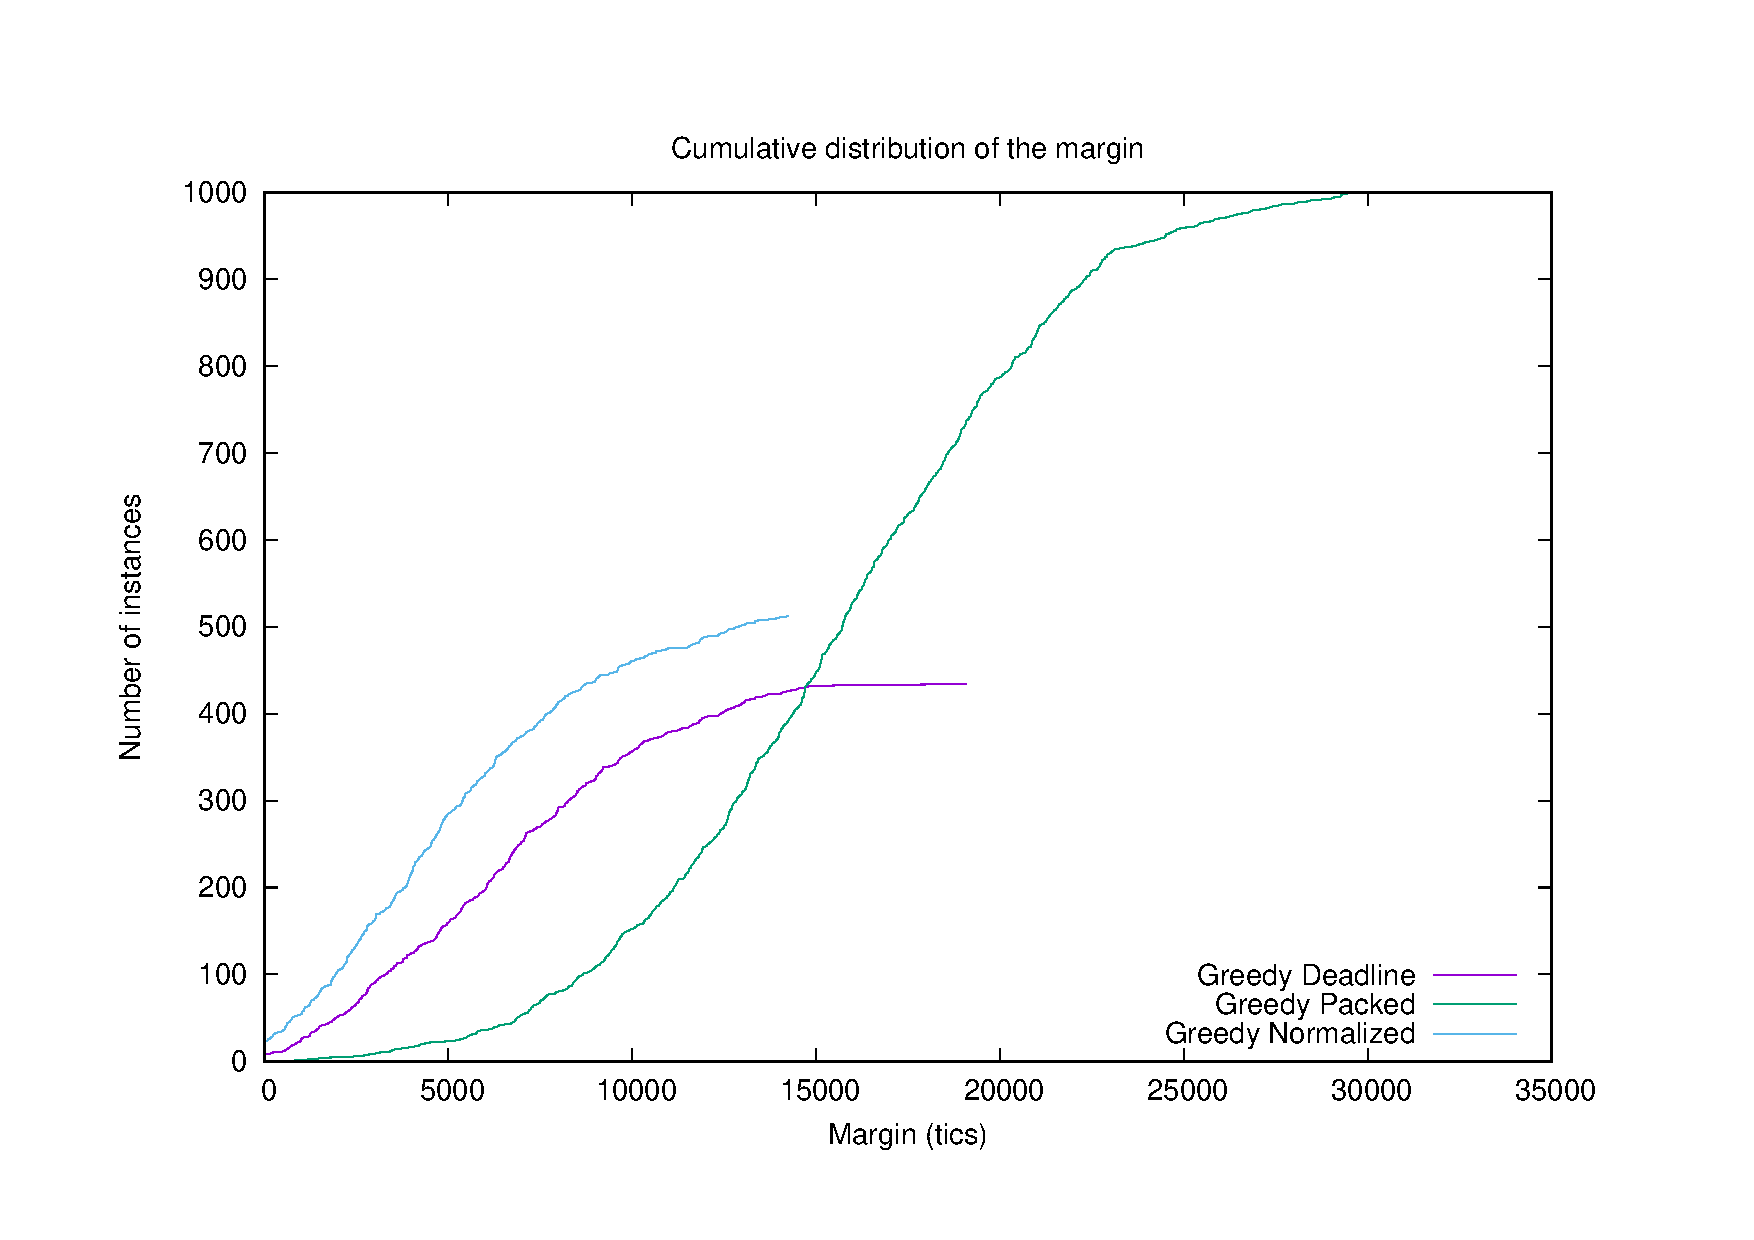
\includegraphics[scale=0.23]{Chapitre5/90load}
\captionof{figure}{Performance of \greedydeadline, \greedynormalized and \greedypacked over $1000$ instances on graphs with $90\%$ load.}
\label{fig:90load}
\end{minipage}
\begin{minipage}[c]{.45\linewidth}
	\centering
	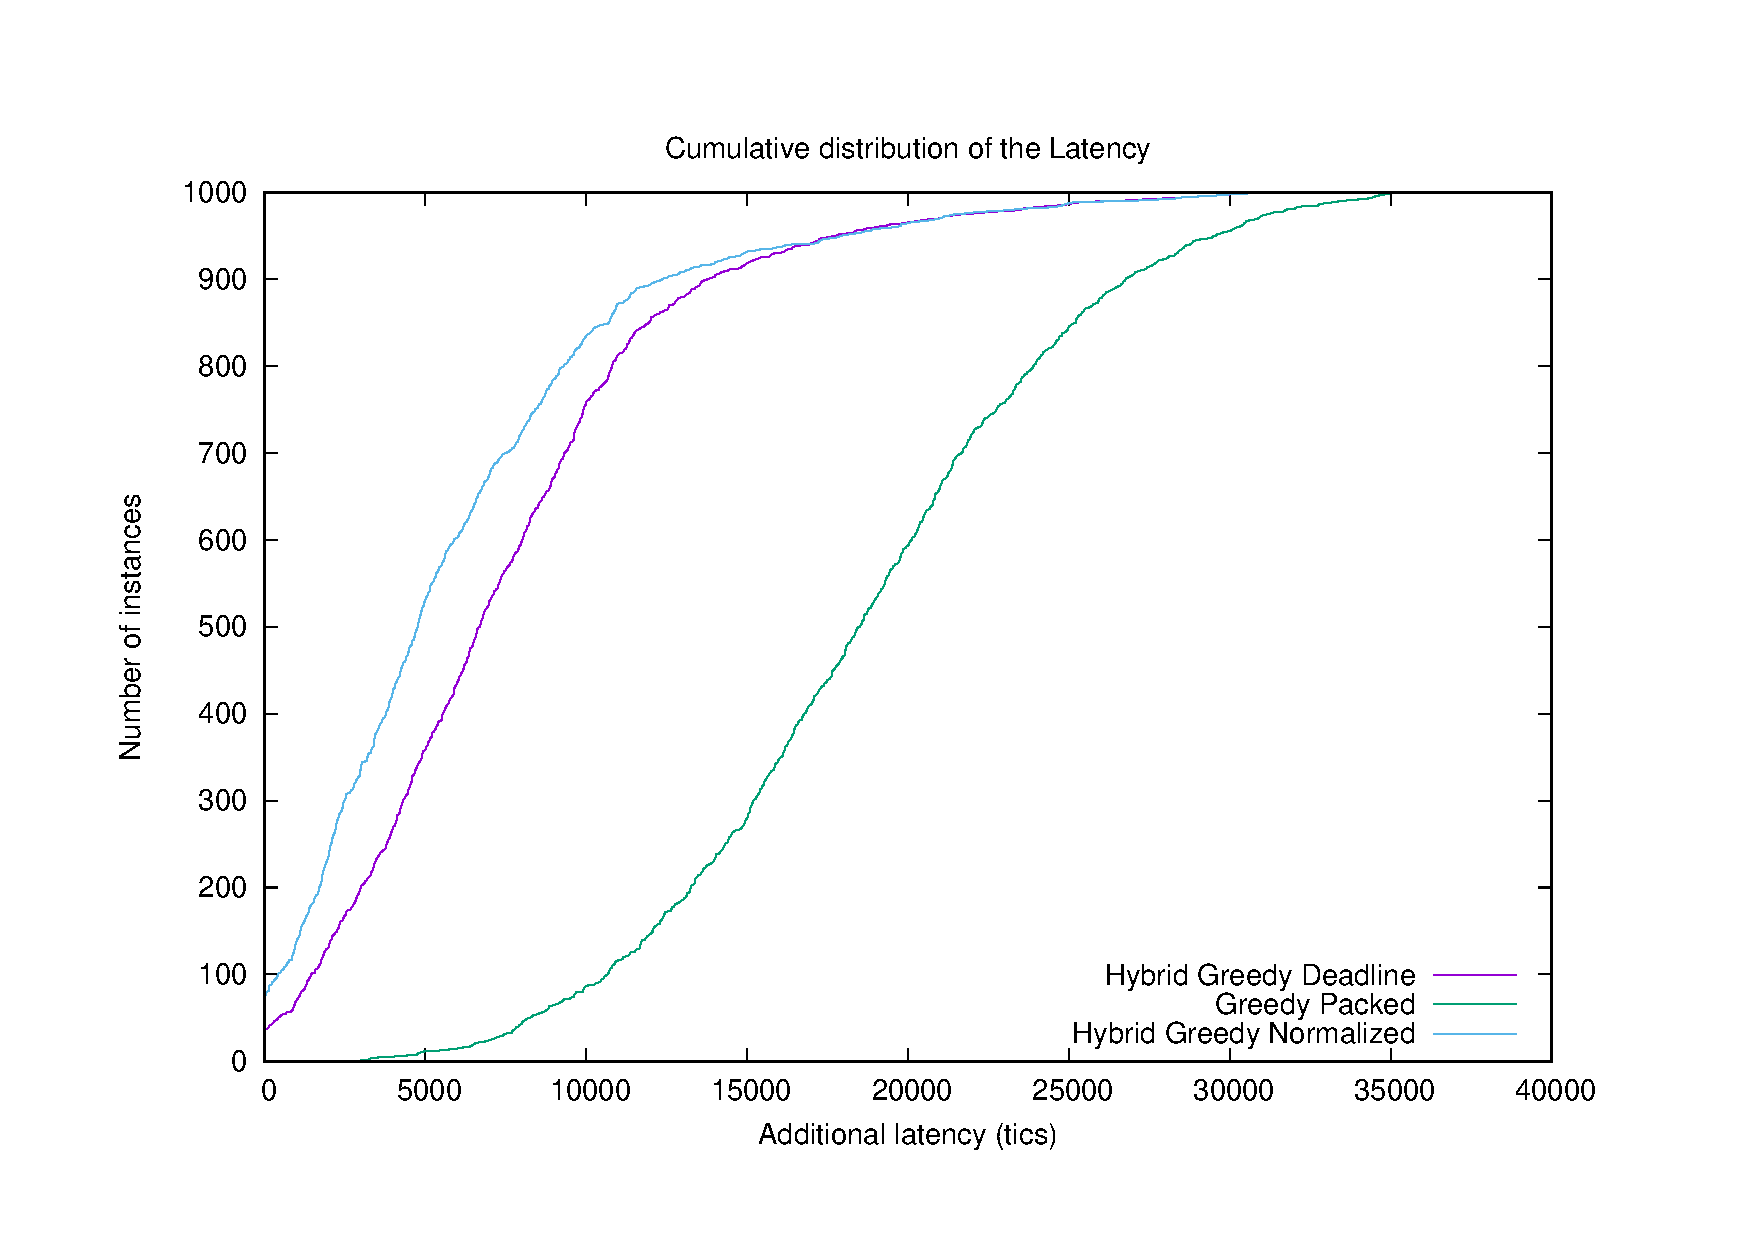
\includegraphics[scale=0.23]{Chapitre5/greedysuccess}
\captionof{figure}{ Performance of the updated greedy algorithms that always gives an assignment} 
\label{fig:greedysuccess}
\end{minipage}

Algorithm \hybridgreedynormalized seems much better than the other two. Hence, in the rest of the paper \hybridgreedynormalized will serve 
as a baseline of assignment quality since it can be obtained in very short time. It will also serve to initialize 
local search algorithms with a first assignment of sufficient quality.

\section{Local Search Heuristics}

The number of compact representations grows extremely quickly with $n$. Hence, to find one which minimizes $TR(A)$, we propose several classical local search algorithm: hill climbing, tabu search and simulated annealing. These methods works as long as a relevant notion of neighborood of a solution is proposed. The neighborood relation must satisfy two properties: it must be quick to compute (hence not to large) and the implicit graph of solutions defined
by the neighborood relation should be connected. We now propose a simple neighborood relation over compact assignments.

Let $u$ be a contention vertex of a network, and let $CA$ be a compact assignment for this network, 
 which associates the pair $(O_u,S_u)$ to $u$. Let $O_u = (r_1,\dots,r_l)$.
  Let $r_i \in \mathcal{R}_u$, the \emph{$r_i$-neighborood} of $(O_u,S_u)$ is the set of pairs $(O,S)$ such that:
 
 \begin{enumerate} 
 \item $O = O_u$ and $S_u = S$ or $S \triangle \{r_i\}$  
 \item $O = (r_1,\dots,r_{i-2},r_{i},r_{i-1},\dots,r_{l})$ and $S_u = S$ or $S \triangle \{r_i\}$ or  $S \triangle \{r_{i-1}\}$ or $S \triangle \{r_i,r_{i-1}\}$ 
 \end{enumerate}

Informally, a compact representation is in the $r$-neighborood of another one if it can be obtained by 
moving down $r$ once (or not changing it) in the order and adding or removing $r$ and the previous route from the set. 
Remark that the $r$-neighborood of any pair $(O_u,S_u)$ has at most $6$ members (it can be $4$ when the route $r$ is in first position and cannot be exchanged with the previous one). 

The \emph{$r$-neighborood} of a compact assignment $CA$ is the set of all compact assignments $CA'=(O'_u,S'_u)_{u \in V(G)}$, such that  $(O'_u,S'_u)$ is in the $r$-neighborood of $(O_u,S_u)$. Finally, the \emph{neighborood} of an assignment $CA$ is the union for all $r \in {\cal R}$ of the $r$-neighboroods of $CA$.

% 
% 
% We define $O(r)$ the position of the route $r$ in an order $O$, and the inverse fuction $O^{-1}(r)$.\\
% We consider a compact represtation $(O_u,S_u)$ on a contention point $u$.
% A \textit{neigbhor order} of  $O$ over a route $r$, is an order $O'$ such that $O'(r) = O(r)+1$ . This means that $O'(j) = O(j),\forall j \notin \{r;O^{-1}(r)+1\}$. Indeed, by definition, $O'(O^{-1}(O(r)+1)) = O(r)$. If $r$ is the last route in the order $O$, then $O'(r) = 1$ and $O'(O^{-1}(O(1))=O(r)$
% A \textit{neigbhor subset} of $S$ over a route $r$ is defined by $S' = S - \{r\}$ if $r\in S$ or $S'= S \cup \{r\}$ if $ r \notin S$.
% The \textbf{neighborhood of the pair} $(O_u,S_u)$ ouver a route $r$ is defined by the set $N_u = \{(O_u,S_u);(O_u,S_u');(O_u',S_u);(O_u',S_u')\}$.\\
% 
% Consider a compact representation $CR(A)$ over a route $r$.
% $CR'(A)$ si a \textbf{neighbor} of $CR(A)$ if for all pair $(O_u,S_u)'$ of $CR'(A)$:
% \begin{itemize}
%  \item If $u \notin r$, $(O_u,S_u)' = (O_u,S_u)$
%  \item If $u \in r$, $(O_u,S_u)' \in N_u $
% \end{itemize}
% 
% The \textbf{neighborhood of a compact representation} $CR$ \textbf{over a route} $r$  is thus the set of compact representations: $\prod_{u\in r} N_u$.
% 
% The \textbf{\underline{neighborhood of a compact representation}} $CR$ is then the set of the compact representations over all routes, that is:
% $$ \bigcup_{r\in{\cal R}} (\prod_{u\in r} N_u ) $$.

 Let us denote by $k_1,\ldots,k_n$ the number of contention vertices on the $n$ routes of 
 a routed network. Then, a compact representation has at most $\sum_{i=1}^n 6^{k_i}$ neighbors. Since the networks we consider are of bounded contention depth ($2$ or $3$ in practice), the size of a neighborhood is linear in the number of routes.  We further restrict the notion of neighborood to realizable compact assignments. Indeed, the unrealizable compact assignments do not yield a real assignment, their transmission time is not defined and we cannot use them in our local search algorithms. We call the graph defined by the neighborood relation over realizable compact assignments of a routed network the \textbf{transposition graph} of the routed network. 
  All algorithms presented in this section will do a walk in the transposition graph, trying to find a vertex with optimal
  transmission time. 

\todo{Faire un dessin d'un routed network simple}


\begin{lemma}\label{lemma:path}
There is a path from a realizable compact representation CR, with $CR(u) = (O_u,S_u)$ to $CR'$, such that 
$CR'$ is equal to $CR$ except on $u$ where it is equal to $(O_u,S_u \cup E)$.  
\end{lemma}
\begin{proof}
The path is by adding elements in $E$ one by one. 
 To prove the existence of the path, it is enough to prove that for  $E = \{v\}$. By definition, $(O_u,S_u \cup{v})$ is in the neighborood of $(O_u,S_u)$. However, one should also prove that $CR'$ is realizable.
  Since the order in which the buffers are fixed by the algorithm of $Real$ is the same for $(O_u,S_u)$ and $(O_u,S_u \cup{v})$, it is easy to prove by induction that the normalized sending times of $(O_u,S_u \cup{v})$ are less than the normalized sending times of $(O_u,S_u)$. Thus, $CR$ realizable implies $CR'$ realizable. Indeed, 
a compact assignment is realizable if and only if the last normalized sending time is less than $P - \tau$.
\end{proof}



 \begin{theorem}
 The transposition graph of a routed network is connected.
 \end{theorem}
 \begin{proof}
 For simplicity, we assume that the routed network has a single contention node $u$. Let $(O_u,S_u)$ and $(O'_u,S'_u)$ be two realizable compact assignments, we show there is a path between them. Let $r$ be the first element of 
$O_u$ and let $E = \mathcal{R}_u \setminus \{ r \}$. By Lemma~\ref{lemma:path}, there is a path from 
$(O_u,S_u)$ to $(O_u,E)$. Consider now $O_u''$, the order $O_u'$ whith $r$ placed in first position.
There is a path from $(O_u,E)$ to $(O_u'',E)$. Indeed, any order is realizable, when all elements but the first
are in $E$ because there are no constraints on their normalized sending time. 
Now, let $r'$ be the first element of $O_u'$. By definition, $(O_u',E \triangle \{r,r'\})$ is in the $r'$ neighborood of $(O_u'',E)$. Moreover, $(O_u',E \triangle \{r,r'\})$ is realizable because $E \triangle \{r,r'\}$ is equal to all routes but the first in $O_u'$. 
Finally, using Lemma~\ref{lemma:path} once again prove there is a path between $(O_u',E \triangle \{r,r'\})$ and $(O'_u,S'_u)$ since $(O'_u,S'_u)$ is realizable and $S'_u \subseteq E \triangle \{r,r'\}$, which proves the theorem.
 \end{proof}




\subsection{Hill Climbing}

The most simple local search heuristic is hill climbing. This algorithm starts from a compact assignment $CA$, explore the entire neighborhood of $CA$, and select the realizable compact assignment $CA'$ of minimal transmission time. Then, we set $CA = CA'$ and repeat this step until there are no $CA'$ such that $TR(CA') < TR(CA)$. Then algorithm stops and returns $Real(CA)$ which is a local minimum. 

The quality of hill climbing depends of the the intial compact assignment. A first natural intialisation is to consider the compact representation $CR(A)$ of the assignment $A$ given by \hybridgreedynormalized. Also, a random compact assignment can be taken. Since a compact assignment does not always give a valid assignment, the last idea is to execetue several hill climbing starting from a random compact assignment, and to return the best assignment given.

Figure~\ref{fig:descente07} shows the difference between initalizing the hill climbing with \hybridgreedynormalized, or with one or several random compact representation. Those resultas are drawn on $1000$ random instances, with $80\%$ of load.
\begin{figure}[h] 
	\centering
	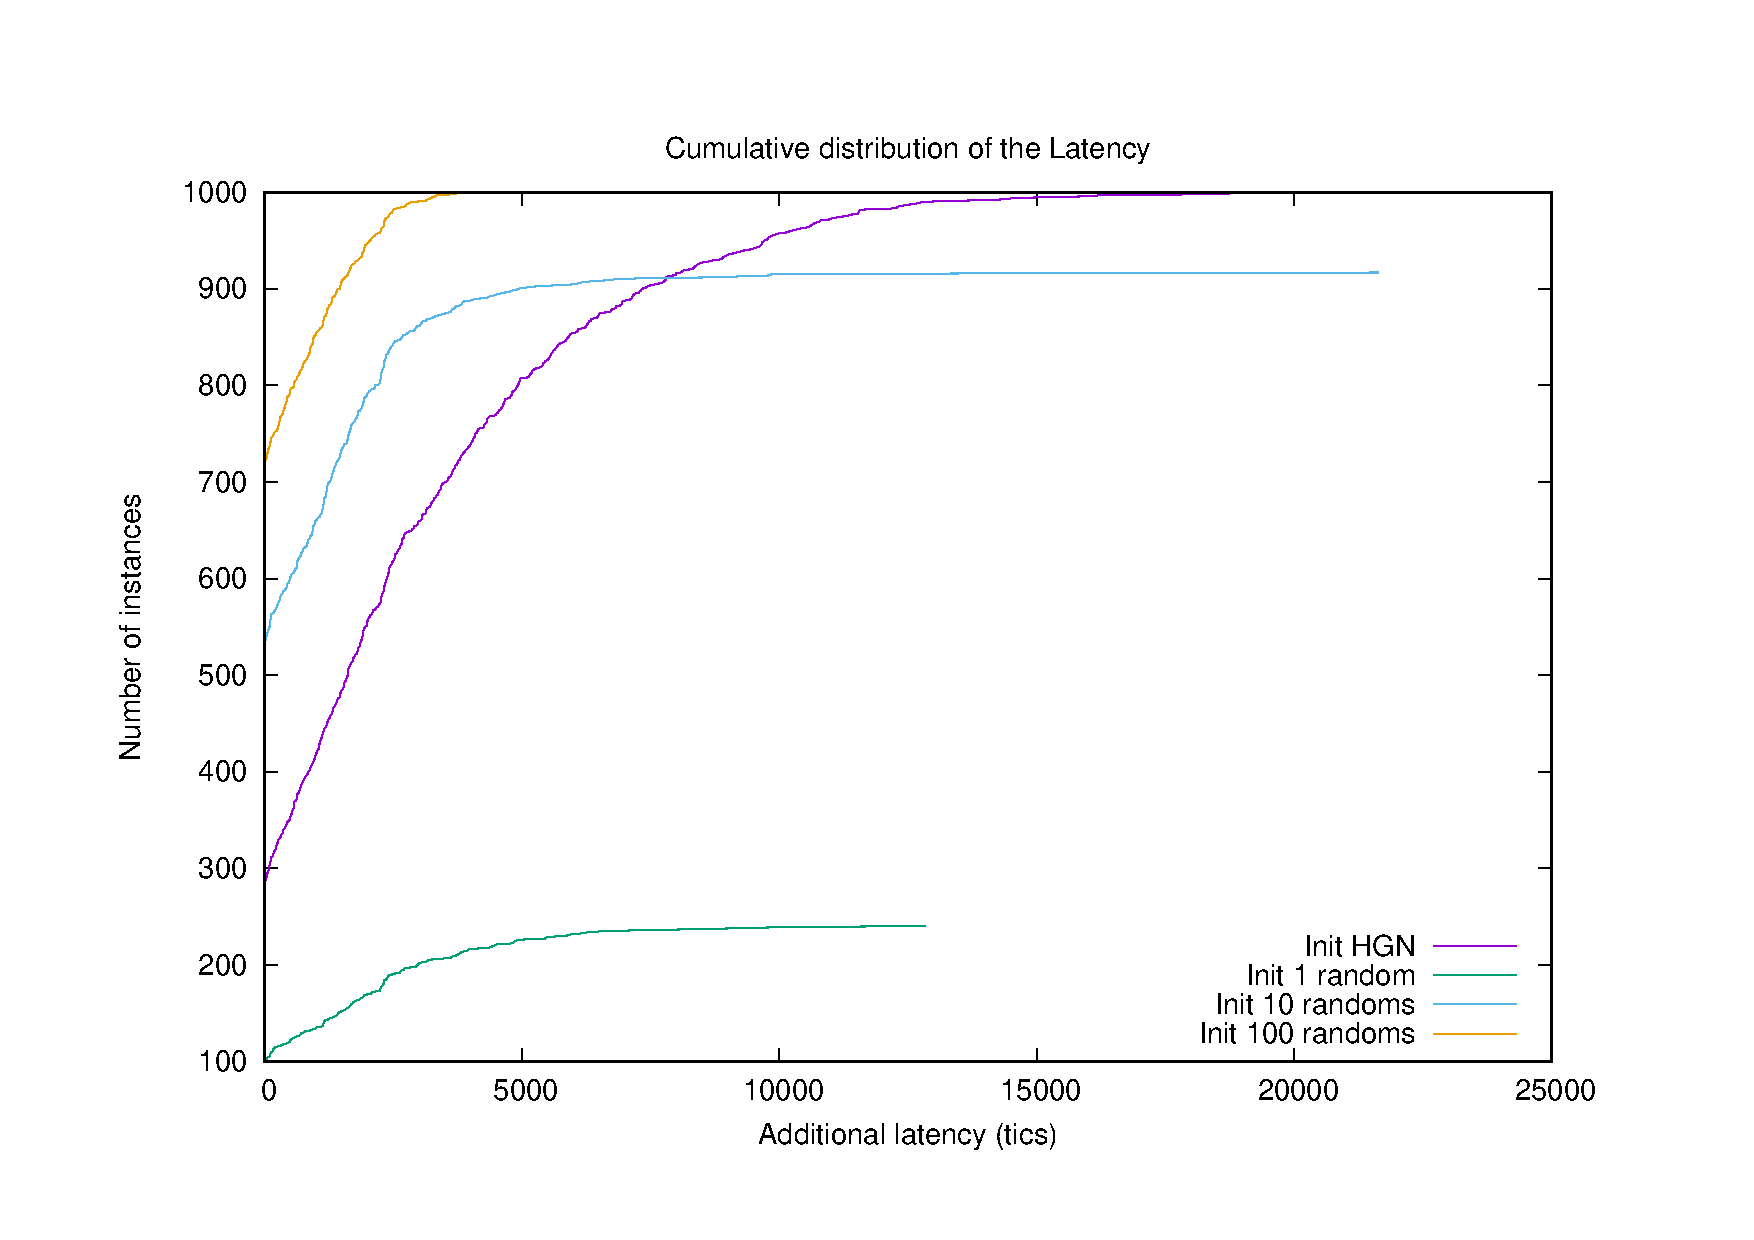
\includegraphics[scale=0.3]{Chapitre5/descente07}
\caption{ Additional latency needed to find a solution for hill climbing, intialized with HGN, 1,10 or 100 random compact representation.}
\label{fig:descente07}
\end{figure}
Initializing the hill climbing with 100 randoms compact representation seems to give better results. Nevertheless remember that the set of compact representation does not always give a valid assignment. Drawing some random compact representation can be a limited option when the set of compact representation grows, because the chance of drawing a non valid, or bad random compact representation grows too.

Figures~\ref{tab:descenteload} and \ref{tab:descentenbroutes} represent the probability of drawing at least one compact representation that gives a valid assignment, when drawing $1$,$10$ or $100$ random compact representations. Each result is computed on $1000$ random instances.

\begin{minipage}[c]{.45\linewidth}
\vspace{-0.4cm}
\begin{tabular}{ |c|c|c|c|c| }
\hline
    Load & $80\%$& $90\%$ & $100\%$\\
    \hline
    HGN & $100\%$ & $100\%$& $100\%$ \\
    1 rand & $7\%$ & $4\%$& $6\%$\\
   10 rand & $49\%$& $42\%$& $28\%$\\
   100 rand & $100\%$ & $97\%$& $92\%$\\
    \hline
 \end{tabular}
   \captionof{figure}{Success rate of hill climbing with different initialization, varying the load.}
 \label{tab:descenteload}
\vfill
 \end{minipage}
 \hfill
\begin{minipage}[c]{.45\linewidth}
\vfill
\begin{tabular}{ |c|c|c|c|c| }
\hline
    Nb routes & $8$& $10$ & $12$\\
    \hline
    HGN & $100\%$ & $100\%$& $100\%$ \\
    1 rand & $7\%$ & $2\%$& $1\%$\\
   10 rand & $49\%$& $23\%$& $5\%$\\
   100 rand & $100\%$ & $86\%$& $56\%$\\
    \hline
 \end{tabular}
 \captionof{figure}{Success rate of hill climbing with different initialization, varying the number of routes on the graph.}
 \label{tab:descentenbroutes}
\vfill
\end{minipage}

Those experiences shows that, even if initializing the hill climbing with $100$ random instances performs well when the number of routes and the load are low, this initialization is not robust when the load of the number of routes increases. Indeed, higher loads induces that good solutions are harder to find, and increasing the number of routes also increase the size of the neighboorhood, and thus, the number of non valid compact representations. Furthermore, the computation time induced by executing the hill climbing on a lot of random compact representation instead of only one (for HGN) makes it less effective.


We thus propose an hybrid initialization of hill climbing: Between the assigments given by initializing the hill climbing either with HGN, or with $1$,$10$ or $100$ random compact representation, return the one that minimize $TR(A)$. We call this initialization respectively hybrid $1$, hybrid $10$ or hybrid $100$.
Figure~\ref{fig:hybridhill} shows the additional latency needed by the best solution given by hill climbing, with different initialisations. The results are computed on $1000$ random instances.
\begin{figure}[h]
	\centering
	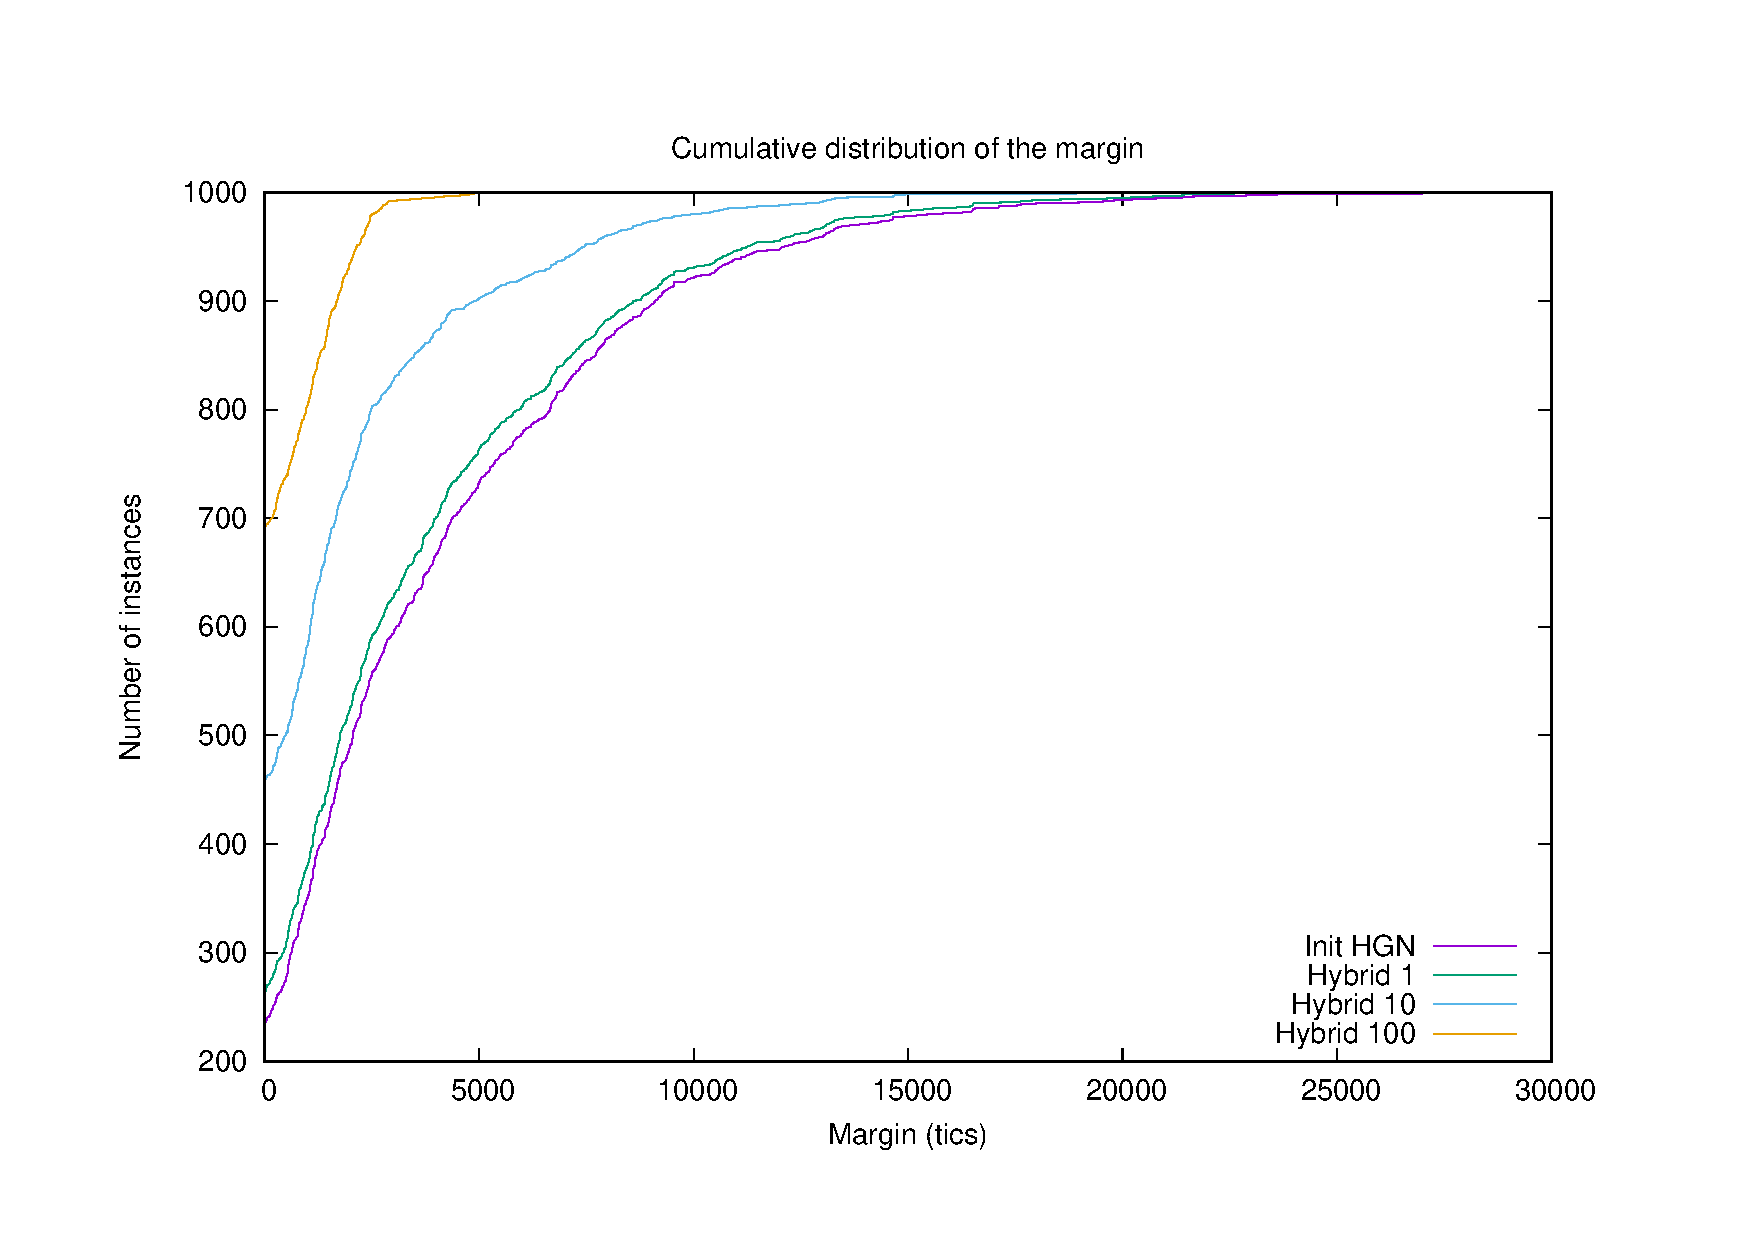
\includegraphics[scale=0.3]{Chapitre5/hybridhill}
\caption{ Additional latency needed to find a solution for hill climbing, intialized with HGN, hybrid $1$, hybrid $10$ or hybrid $100$.}
\label{fig:hybridhill}
\end{figure}

We now focus on how many steps hill climbing computes before ending. Tabular~\ref{tab:nbstepdescente} shows the average number of steps of the hill climbing with different initializations. Those results come from the experiment of figure~\ref{fig:hybridhill}.

\begin{tabular}{ |c|c|c|c|c| }
\hline
    Init & HGN& Hybrid $1$& Hybrid $10$& Hybrid $100$\\
    \hline
    Average Nb Step & $1.14$ & $1.26$& $1.92$&$3.38$ \\

    \hline
 \end{tabular}
  \captionof{figure}{Average number of step needed by hill climbing to reach a local optimum.}
 \label{tab:nbstepdescente}

 The more the hill climbing does steps before ending, the more the initial solution is improoved. When hill climbing starts from a \hybridgreedynormalized, it does not improove often the solution whereas with a huge number of random compact representation, the probability of drawing a solution that can be improoved a lot is increased.
 
 The concept of drawing a large number of random compact representation to initialize the hill climbing link with the concepts of taboo search and simulated annealing. Indeed, the two next meta-heuristics are designed to explore the compact representations, even if a local optimum is reached. Taboo remembers the explored solutions, in order to avoid it, and simulated annealing browse the compact representations with a stochastic aspect.
\subsection{Tabu Search}

Tabu search is a variation on hill climbing using memory. We also select the compact assignment $CA'$ which minimizes 
$TR(CA')$, even when $TR(CA') < TR(CA)$ is not satisfied. To avoid loop in local minimum, we use a memory of the last 
$N$ solutions explored and we forbid to visit them again. This algorithm can still loop on a cycle larger than $N$,
hence we must fix some integer $M$ and stop the algorithm after $M$ steps.


One can change the size $N$ and $M$ in tabu search -> explore how to fix these parameters. 

After reaching a local optimum, tabu search continues it execution untill it has executed a given number of steps.
Thus, we investigate the average number of steps needed by the tabu search to find the assignment it returns. Remember that, to each step, the search explores the entire neighborhood of a solution. The computation of a large number of steps is then long.

Tabu search has a memory, it remembers the compact assignment for which it explored the neighborhood for the $x$ last solutions in order to not visit them again. Varying the value of $x$ can improve or worsen the performance of the tabu search.
Figure~\ref{fig:tabudistrib} shows cumulative distribution of the additional latency needed by tabu search with different size of memory. The number of steps computed by the tabu search is $1000$.
\begin{figure}[h]
	\centering
	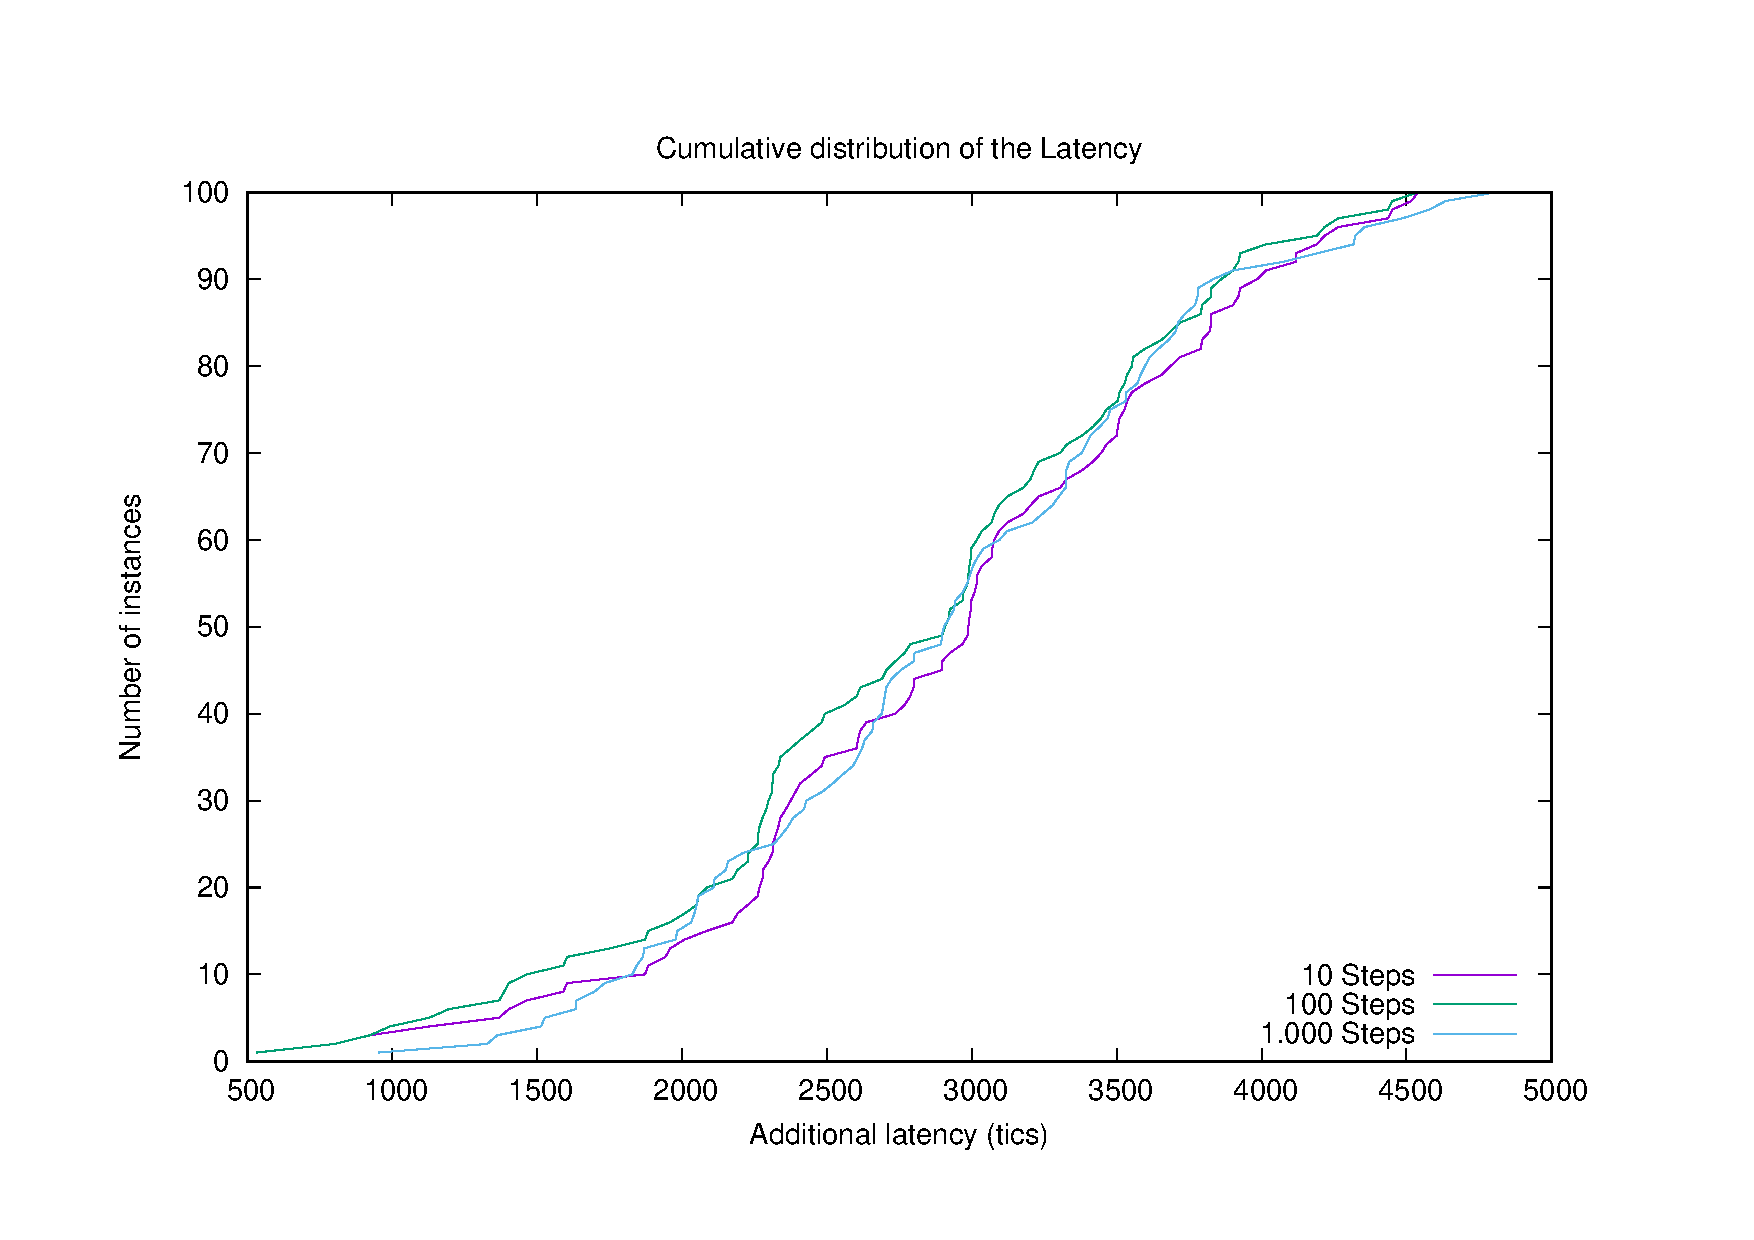
\includegraphics[scale=0.3]{Chapitre5/taboo_distrib}
\caption{ Difference between the tabu search whith a memory of $10$,$100$ or $1000$ solutions}
\label{fig:tabudistrib}
\end{figure}
It appears that, the more steps tabu search remember, the better the assignment given is.
In order to understand what happends during the tabu search, we investigate the distribution of the step at which the tabu search finds its best solution.
For $10$ steps of memory, tabu search finds the best assignment in average in $3.8$ steps, with a memory of $100$ steps, the average step that gives the best assignment is $18.1$, and for $1000$ steps, tabu search needs in average $84.3$ steps to find the best solution. 
Also, it appears that, in most of $60\%$ of the cases, tabu search finds it's best assignment before $10$ steps, but some computation finds a better assignment up to the $900^{th}$ step. This means that running the tabu search longer could improove the quality of the result. Nevertheless, this the computation is really expensive, using simulated annealing is more interesting.

\subsection{Simulated annealing}

Simulated annealing works as follow. An initial {\emph temperature} is set and an initial compact representation is chosen. At each step, we try to replace the current valid compact representation $CA$, by $CA'$ drawn unfiformly at random in the neighborood of $CA$. Then, using the temperature, $TR(Real(CA))$ and $TR(Real(CA'))$, $CA'$ is either accepeted or rejected. After a given number of steps, the temperature is decreased by multiplying it by some constant less than one. The lower the temperature, the lower the chance to accept a compact assignment that worsen the solution. The algorithm is an anser to the exploration/exploitation paradox: in the beginning of the algorithm the whole solution space is explored but as the temperature decreases, the search becomes more and more local around a good solution.

 When using simulated annealing, we need to fix several parameters: initial temperature, number of steps before decreasing the temperature, factor by which the temperature is decreased, the number of steps without improvement before ending the process.

 \todo{ During the computations $1000$ compact representation are drawn before decreasing the temperature.
 Mettre aussi par quel facteur tu diminues la température et ta condition d'arrêt}

 The temperature must be fixed in order to accept to worsen the solution at the begining of the execution, must decrease slowly. When the temperature is low, the simulated annealing rejects bad compact representations.
 Accepting or rejecting a solution is a stochastic process. Consider $CA$, the best compact assignment found during the exection of the simulated annealing. The value $\Delta$ represent the difference $TR(REAL(CA'))-TR(REAL(CA))$ where $CA'$ is a compact assignment in the neighboorhood of $CA$. $CA'$ is accepted or rejected with the probability $e^{-\frac{\Delta}{t}} $, where $t$ is the temperature.
 This means that $\frac{\Delta}{t}$ must be close to $0$ at the begining, and must approaches infinity at the end of the execution. 
 
 In order to fix the initial temperature $t_0$, we follow~\cite{osman1997meta}:
 \begin{enumerate}
  \item Initiate 100 disturbances at random; evaluate the average $\bar{\Delta}$ of the corresponding variations $\Delta$
\item Choose an initial rate of acceptance $\tau_0$ of the “degrading perturbations” according to the assumed “quality” of the initial configuration; for example:
\begin{itemize}
 \item “poor” quality: $\tau_0 = 50 \%$ (starting at high temperature)
\item “good” quality: $\tau_0 = 20 \%$ (starting at low temperature)
\end{itemize}


\item Deduce $t_0$ from the relation: $e^{-\frac{\bar{\Delta}}{t_0}} = \tau_0$ 
 \end{enumerate}
 
 Tab.~\ref{tab:poorgood} shows the additional latency of the solutions produced by simulated annealing when intialized with temperatures computed from the previous routine. The initial solution used by simulated annealing is the solution given by $0$-HHC. The experiment is made on $100$ random instances.
\begin{center}
\begin{tabular}{ |c|c|c|c|c| }
\hline
 Quality of initial configuration & Good& Poor\\
    \hline
    $t_0$ & $2200$& $13000$\\
    \hline
    Additional latency & $4212$ & $4217$ \\
        \hline
    Computation time (ms) &  $2.817$&$4.035$ \\

    \hline
    
 \end{tabular}
 \caption{Comparison of two intial temperatures, considering the quality of the initial configuration}
     \label{tab:poorgood}
 \end{center}
 As observed, the initial solution given by hill climbing can be considered as ``good''. Indeed, increasing the initial temperature does not affect the quality of the solution, but increase the computation time.
 
 In simulated annealing, the temperature decrease slowly. Each \textbf{level}, several compact representation are drawn. At the end of a level, the temperature is decreased. Drawing too few compact representation per level induce decrasing the temperature too fast and thus, reducing the efficiency of simulated annealing. In an ohter hand, drawing too much compact representation increases the computation time of the algorithm.
  
 We investiage the impact of drawing a large number of compact representation before decreasing the temperature. Figure~\ref{fig:stepsrecuit} shows the additional latency needed by simulated annealing with different number of compact representation draw for each level. Those results comes from $1000$ random instances, in which the temperature is set to $2200$.
 
 \begin{figure}[h]
	\centering
	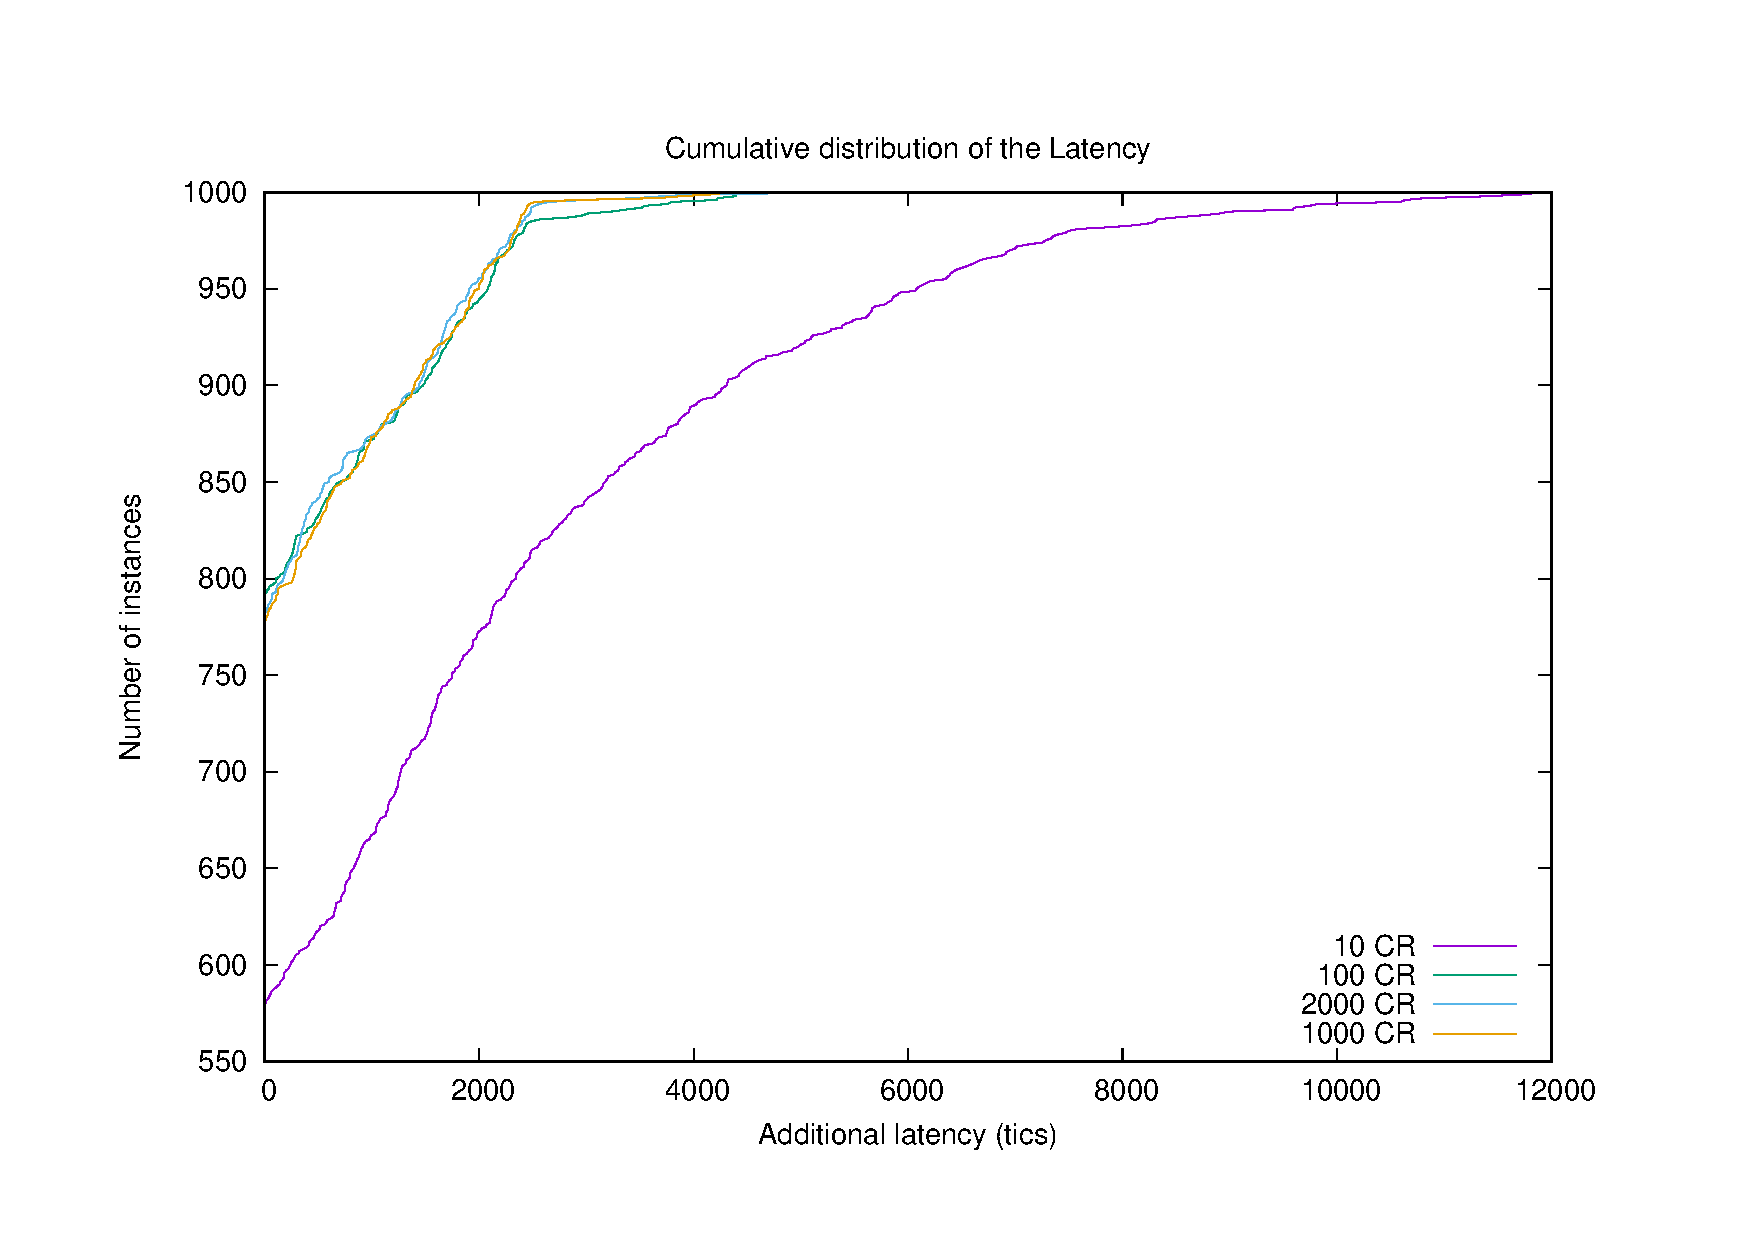
\includegraphics[scale=0.4]{Chapitre5/stepsrecuit}
\caption{ Additional latency needed to find a solution for simulated annealing, with a different number of compact representation drawn to each level.}
\label{fig:stepsrecuit}
\end{figure}
It appears that drawing more than $100$ compact representation per level does not improove the quality of the solution, while it increase the computation time.

\todo{differents profils de temperature}
 

\section{Branch and Bound}

\subsection{Partial Compact Assignment and Relaxation}

D'abord introduire la notion de solution partielle avec seulement les temps d'attente fixée
sur seulement une partie des sommets de contention (dans l'ordre des niveaux de contention).

Puis définir le graphe associé à une solution partielle, en enlevant les sommets déjà traités 
et en mettant à jour les délais. Un exemple serait le bienvenu.

Donner la relaxation du problème général au problème sur un point de contention, 
c'est à dire remplacer tous les chemins vers et depuis le sommet par un arc de la même longueur.
Expliquer que la solution optimale pour le problème relaxé est meilleure (borne supérieure) de
ce qu'on cherche. On définit ensuite une borne supérieure meilleure en faisant le max des 
relaxations pour tous les points de contention. Expliquer que cette borne se calcule facilement
en pratique (algo Simmons FPT vs algo branch and bound simplifié).
\subsubsection{Partial Compact Assignment and restricted routed Network}

Let us consider the contention points ordered from $0$ to $|{\cal C}|$ by contention level, and an arbitrary order is set in a same contention level. This means that if $i < j | i,j\in{\cal C}$, then  $cl(c_1) \leq cl(c_j)$. 


Let us denote $CA|i$ the \textbf{partial Compact Assignment} function. This is the restriction $CA:[{\cal C}]\nrightarrow[i]$ of the domain of definition of $CA$ from $[{\cal C}]$ to $[i]$. This means that a couple $(O_{c_j},S_{c_j})$ has been set only for $j \leq i$.

A \textbf{restricted routed Network} is defined by $N_i = (CA|i,{\cal R}',{\cal C}',\omega')$. It is a routed network $N = ({\cal R},{\cal C},\omega)$ modified by a partial compact assignment $CA|i$.
Let us explain how to build $N_i$ from $N$ and $CA|i$.
Consider that $CA$ is defined only on the first contention point $c_1$ on a routed network $N$.
A route $r = (s,c_1,c_2,\ldots,t)$ in ${\cal R}$ becomes $(s,c_2,\ldots,t)$ in ${\cal R}'$ and $\omega'(r,s) = \omega(r,s)+\omega(r,c_1) + A(r,c_1)$. Indeed, as explianed on Section~\ref{sec:real}, the function $Real$ can be independently computed on each contention points of contention level $1$, then on each contention points of level $2$ etc. Thus, we can compute $Real(CA|1)$ that gives $A(r,c_1)$ for each $r \in {\cal R}_{c_1}$. Also, since $c_1$ is not considered anymore in $N_i$, ${\cal R}' = {\cal C} \backslash {c_1}$\\
This transformation can be repeated on each contention points for which $CA$ is defined, because, as we defined, the contention points are ordered by increasing contention level.

\subsubsection{Relaxation on a single contention point}

In order to describe the Branch and Bound Algorithm on the next section, we need to be able to compute an lower bound for $TR(A)$.
We show here how to transform an instance of \spall into an instance on a single contention points, which is the problem \wta solved in Chapter~\ref{chap:PALL}. 

Consider the routed network $N = ({\cal R},{\cal C},\omega)$. We want to compute an upper bound of $TR(A)$ with $A$ the optimal solution for \spall. 

We describe here how to relax an instance $I$ of \spall with a routed network $N$, and deadline function $d$ into an instance $I'$ of \wta. 
To transform $I$ into $I'$, we focus on one contention point (let us take $c_1$, the first one) of the routed network $N$. Remeber that an instance of \wta consists in a size of messages $\tau$, which is the same as in $I$, a set of routes wich is here ${\cal R}_{c_1}$, a release function, which is here the arrival time $t(r,c_1)$ and a deadline function $d'$. The arrival time is computed from $Real(CA|1)$.
We consider there is no other contention points than $c_1$ in the rest of the network. Then, for all $r \in {\cal R}_{c_1}$, $d'(r) = d(r) - \lambda(r) - t(r,c_1) + \lambda(r,c_1)$. The deadline now correspond to the margin of previous chapter.
Such a relaxation can be done on every contention point $c_i$ for which $CA|j$ is defined, with $cl(j)<cl(i)$ . In other words, if $CA$ is defined on all contention points of a same level (let's say $k$), it is possible to build an instance of \wta for each contention points with a contention level lower or equal to $k$. Indeed, it is possible because we can compute $t(r,c_i)$.



Thus, considering $CA|i$, one can compute a lower bound for $TR(Real(CA|i))$. First, build an instance $I'$ of \wta for each contention points as defined above. Then, use \ASPMLS to find an optimal assignment $A'$ that solve $I'$ in time $O(2^nn^3\log(n))$, where $n$ is the number of routes. By taking the maximum between all $TR(A')$, we thus have a lower bound for $TR(Real(CA|i))$.


\subsection{The Branch and Bound Algorithms}


To solve \spall, we need to find an assignment for which $TR(A)$ is minimal. 
To do so, because of Lemmas of Section~\ref{sec:real}, it is enough to 
enumerate all canonical compact representations, to compute their realization and the corresponding transmission time.

\begin{theorem}\label{theorem:FPT}
For routed networks of fixed contention depth $d$, the problem \spall parametrized by $n$ the number of routes is FPT: it can be solved in time $O(nd(n!2^{n})^{d})$.
\end{theorem}
\begin{proof}
The algorithm to solve \spall is the following: all compact assignments $CA$ are generated, for each of them $TR(Real(CA))$ is computed in time
$O(nd)$ by Lemma~\ref{lemma:canonical} and we keep the compact assignment for which this value is minimal.  Because of Lemma~\ref{lemma:prec}, to compute the minimum of $TR(A)$, it is enough 
to compute the minimum of $TR(Real(CA))$.

 Now, we need to evaluate the number of compact assignments. 
On a single contention vertex $u$ with $s = |\mathcal{R}_u|$ routes going through, there are $s!2^s$ possible restrictions of a compact assignment by counting the number of pairs of set and order over $\mathcal{R}_u$.
On a given contention level consisting in the vertices $\{u_1,\dots,u_l\}$, with $s_i = |\mathcal{R}_{u_{i}}|$, there are 
$\prod_{1 \leq i\leq l} s_i!2^{s_i}$ compact assignments. On a given contention level, all routes use at most $1$ vertex, hence $\sum_{1 \leq i\leq l} s_i \leq n$. Since $\prod_{1 \leq i\leq l} s_i! \leq (\sum_{1 \leq i\leq l} s_i)!$, we have $\prod_{1 \leq i\leq l} s_i!2^{s_i} \leq n!2^n$. There are $d$ contention levels, thus we have at most $ (n!2^{n})^{d}$ compact assignments which proves the theorem.
\end{proof}

Note that for the vertices of the last contention level, compact assignments can be considered independently, since
they do not interact. Hence, if the last level contains the vertices $\{u_1,\dots,u_l\}$, we only need to consider $(n!2^{n})^{d-1}(\sum_{1 \leq i\leq l} s_{i}!2^{s_i})$ assignments. This makes a large difference in our target application and the experiments presented in this chapter, since in this context $d$ is two or three and the $s_i$'s are pretty balanced.
\todo{dire qu'on peut encore plus faire baisser la complexité en utilisant not simmons FPT à ce niveau. Enfin analyser le nombre de solutions qu'on voit en ne regardant que les canoniques,
(minimales ?)}

Définir l'arbre de recherche exhaustif sur les solutions partielles et expliquer les coupes
qu'on peut faire grâce à la borne sup qu'on vient de définir (en gardant la valeur de la meilleur solution
et en initialisant cette valeur par un algo de bonne qualité, genre hill clibming ou carrément recuit simulé).


\subsection{Locally minimal representation}

On voudrait énumérer uniquement les solutions qui sont minimales pour 
$\prec$ pour un sommet donné et canoniques, ce qu'on appelle des solutions locally minimal.

On propose un ensemble de coupes faciles à calculer qui permettent d'éliminer la plupart des solutions 
non minimales. Proposer une caractérisation des solutions localement minimales (à vérifier).

Montrer avec des expériences (nombre de représentation générées et pourcentage de minimales en fonction du nombre de routes) que ces coupes sont très efficace, elles permettent de générer uniquement des représentations compactes canoniques valides, et presque aucunes dont la réalisation n'est pas minimale.

\subsection{Last Contention Level}

Mettre ici le traitement spécifique du dernier niveau -> analyse de la complexité différente 
à mettre ici, certaines coupes à ne pas faire car seul l'objectif de temps global nous importe 
(à vérifier c'est un tradeoff, mais certaines sont évidemment à retirer). 


\section{Experimental Evaluation}

Comparer les temps de calcul et la qualité des solutions trouvées. 
Le faire pour plusieurs régimes:
-8 routes vs bcp de routes (branch and bound impossible)
-charge 40 80 et 100 pour cent
-routes dont les arcs sont tous petits (tirés dans [tau] ou moins) ou grands (tirés dans [P]).
-plus de 2 data centers, 3 ou 4 ?

Enfin comparer aux méthodes de multiplexage statistique avec FIFO et Greedy Deadline.
Expliquer les rapports/différences de ces méthodes avec les algos greedys.



\section{Autres trucs à raconter ?}
Once all those synthetic datas are set, we focus on the length of the arcs in the grap. We look at three ways to draw some values for the length of the arcs: uniformly between $0$ and $\tau/3$ (with $\tau$ the size of a datagram), uniformly between $0$ and $P$ (the size of the period), and uniformly between $P-0.1\times P$ and $P$.
\todo{expliquer pourquoi ces valeurs}

Figure~\ref{tab:instances} shows the average additional latency needed by the branch and bound and the greedy algorithm that we call HGN presented in next section (used to intialize the local search algorithms) for the different ways to draw the length of the arcs. Those values are draw for $100$ instances of each kind.

\begin{center}
\begin{figure}
\centering
\begin{tabular}{ |c|c|c|c|c| }
\hline
    Range & $0$ and $\tau/3$ & $0$ and $P$& $P-0.1\times P$ and $P$\\
    \hline
    Branch and bound & $4273$ & $222$& $2704$ \\
 
    HGN & $12177$ & $10628$& $9648$\\
   
    \hline
  
 \end{tabular} 
 \caption{Difference between the optimal solution of the greedy algorithms, for different kind of instances generated.}
 \label{tab:instances}
 \end{figure}
 \end{center}
 The objective is to find the instances in which a solution given can be the most improoved by the local search heuristics. As observed, when drawing the size of the arcs betwenn $0$ and $P$, the lower bound (found by the branch and bound algorithm) is clearly lower than with the other kinds of instances while the additional latency needed by HGN remains in the same order of magnitude.
 